% Template for PLoS
% Version 1.0 January 2009
%
% To compile to pdf, run:
% latex plos.template
% bibtex plos.template
% latex plos.template
% latex plos.template
% dvipdf plos.template

\documentclass[10pt]{article}

% amsmath package, useful for mathematical formulas
\usepackage{amsmath}
% amssymb package, useful for mathematical symbols
\usepackage{amssymb}

% graphicx package, useful for including eps and pdf graphics
% include graphics with the command \includegraphics
\usepackage{graphicx}
\usepackage[utf8]{inputenc}
\usepackage[T1]{fontenc}
\usepackage[icelandic,english]{babel}
\usepackage{float}

% cite package, to clean up citations in the main text. Do not remove.
\usepackage{cite}

\usepackage{color} 

% Use doublespacing - comment out for single spacing
%\usepackage{setspace} 
%\doublespacing


% Text layout
\topmargin 0.0cm
\oddsidemargin 0.5cm
\evensidemargin 0.5cm
\textwidth 16cm 
\textheight 21cm

% Bold the 'Figure #' in the caption and separate it with a period
% Captions will be left justified
\usepackage[labelfont=bf,labelsep=period,justification=raggedright]{caption}

% Use the PLoS provided bibtex style
\bibliographystyle{plos2009}

% Remove brackets from numbering in List of References
\makeatletter
\renewcommand{\@biblabel}[1]{\quad#1.}
\makeatother


% Leave date blank
\date{}

\pagestyle{myheadings}
%% ** EDIT HERE **


%% ** EDIT HERE **
%% PLEASE INCLUDE ALL MACROS BELOW

%% END MACROS SECTION

\begin{document}

% Title must be 150 characters or less
\begin{flushleft}
{\Large
\textbf{Measles in small populations : predictability in highly stochastic systems}
}
% Insert Author names, affiliations and corresponding author email.
\\
Q. Caudron$^{1,\ast}$, 
A. S. Mahmud$^{2}$, 
C. J. E. Metcalf$^{1}$,
M. Gottfre{\dh}sson$^3$,
B. T. Grenfell$^{1}$
\\
\bf{1} Department of Ecology and Evolutionary Biology, Princeton University, Princeton, NJ, 08544, USA
\\
\bf{2} Office of Population Research, Woodrow Wilson School of Public and International Affairs, Princeton University, Princeton, NJ, 08544, USA
\\
\bf{3} Landsp\'{i}tali, Hringbraut 101, Reykjav\'{i}k, Iceland
\\
$\ast$ E-mail: qcaudron@princeton.edu
\end{flushleft}













% Please keep the abstract between 250 and 300 words
\section*{Abstract}

A standard assumption in the modelling of epidemic dynamics is that of a certain level of homogeneity. In childhood infections, such as measles, populations are typically assumed to be large and well-mixed, and the data assumed to contain a high signal-to-noise ratio. This allows the use of differential equations as a model for disease dynamics, generally with positive results, both in terms of explaining the underlying mechanisms for infection, and for the prediction of future time series data on disease incidence. Here, we consider a setting where populations are small and heterogeneous, and where the dynamics of infection are driven by extinction-recolonisation events. Using a TSIR model, we fit prevaccination measles incidence and demographic data in Bornholm, the Faroe Islands, and four districts in Iceland, between 1901 and 1965. We explore the potential for prediction in this model : given historical incidence data and up-to-date demographic information, and knowing that a new epidemic has just begun, can we predict how large it will be ? We show that, despite a lack of significant seasonality in the incidence of measles cases, we are able to estimate the size of upcoming epidemics, conditioned on the first time step, to within reasonable confidence. Reporting rates are estimated to vary widely over time

Each of these countries are characterised by a different level of data heterogeneity












\section*{Introduction}

Needs padding and fixing...

Measles is a highly contagious and strongly immunising infection of the respiratory system. Due to its extreme transmissibility, its epidemiology is conditional on the birth of susceptible individuals. As such, the temporal dynamics of measles are typically strongly oscillatory, driven seasonally by the increased contact rate amongst children during school periods, assuming the population is large enough to sustain the disease (Black FL, 1966, JTB 11). These dynamics have been well studied (Grenfell papers, others), and many modelling efforts have successfully explained the biennial cycle exhibited in prevaccination records of measles incidence in Europe and elsewhere (papers ?). 

In small populations, where the number of individuals is much smaller than the critical community size required to support an endemic infection, however, the dynamics of measles cases are vastly different. Susceptible individuals accumulate when measles is absent; then, driven by stochastic importation, an epidemic may sweep through a large fraction of the susceptible population very quickly, only to go extinct abruptly as susceptibles become depleted. This results in very sharp, spiky epidemics, the timing of which may be impossible to predict, but the size and duration of which may be a function of historical data. 

In this paper, we address the question of predictability of measles epidemics in small populations, based on records of past incidence and on demographic data. We present data on the demographics and disease incidence in prevaccination-era Bornholm, the Faroe Islands, and four districts in Iceland. 

reconstruct the dynamics of susceptible individuals and infer the rate of reporting of cases using the TSIR model (Finkelstadt and Grenfell 2000) in prevaccination 
 
	

sizes are, by training a model on records of past epidemics and demographic data. Using the TSIR model (Finkelstadt and Grenfell, 2000), we explore the dynamics of measles in prevacinnation Bornh


Any seasonality ? 






\section*{Methods}

\subsection*{Raw Data}

Measles incidence data were obtained for Iceland, the Faroe Islands, and Bornholm (CONFIRM?), from 1900 to 1965, from \citet{Cliff1983A}. For Iceland, this dataset collects monthly figures for measles cases reported in 47 medical districts, originally sourced from Heilbrigdisskyrslur (Public Health in Iceland). Major revisions to the boundaries of medical districts took place twice during the study period : in 1907 and 1932. For the Faroe Islands and Bornholm, the data were originally published WHERE?. 

Demographic data for Iceland were obtained from two sources. Annual data on population and number of live births for the entire country were taken from \citet{Cliff1983B}. Decadal population data from 1901 to 1965, for 262 municipalities, were obtained from online publication in \citet{StatisticsIceland}. Municipality boundaries changed from three to five times during the study period. In addition, many municipalities had missing data. Medical districts and municipalities were matched based on names, and confirmed using latitude and longitudes. Using this procedure, we were able to confidently match four medical districts with municipalities. Several matched districts were discarded either due to missing population data, or lack of confidence in the matching of the geographical boundaries. It is also worth noting that matched medical district - municipality pairs may not encompass the exact same area, but one may be a (potentially partial) subset of the other.

Data on the demographics of the Faroe Islands were taken from the Statistical Yearbooks of Denmark published by \citet{StatisticsDenmark}. Annuak data on population and births from 1901-1965 were obtained in aggregated form for all of the islands in the Faroe archipelago. 

Demographic data for Bornholm was collected from several publications from \citet{StatisticsDenmark}. Annual population data for Bornholm were obtained from \citet{StatBankDenmark}, which contains detailed statistical information collected by Statistics Denmark. Pre-1930 annual birth data were obtained from the �\UTF{00C6}gteskaber, F\UTF{00F8}dte og D\UTF{00F8}de� (Marriages, Births and Death) publications of Statistics Denmark. POS930 annual birth data were obtained from �Befolkningsudvikling og sundhedsforhold 1901-60� (Population, Development and Health 1901 \UTF{2013} 1960). CITE URLs.

All locations experienced a slight decline in birth rates just prior to 1940, followed by a sharp increase in births after 1940. In Bornholm, births declined steadily from around 1945 onwards. In Iceland and the Faroe Islands, aggregate births increased steadily from 1940s onwards, with a slight decline in Iceland around 1960.






\subsection*{Data Preparation}

In order to 




Interpolation


Demo description : 
How births were calculated; all births in Iceland drop from 1930 - 1940 then baby boom





Data very spiky, monthly. Interpolated two points per point ( not quite biweekly, 24 periods ). Qualitatively : Iceland spiky, Bornholm smoother, Faroe lots of small epis. 








\section*{Model}

\begin{align}
I_{t} &= r_{t} \, I_{t-1}^\alpha \, S_{t-1} \, \varepsilon_t \\
S_{t} &= B_{t-d} + S_{t-1} - I_{t-1}
\end{align}

\begin{equation}
I_t = \rho_t \, C_t
\end{equation}


\begin{align}
S_t = \bar{S} + Z_t
\end{align}

% Results and Discussion can be combined.
\section*{Results}

\begin{figure}[H]
\label{fig_timeseries}
\caption{\textbf{Reported incidence and inferred reporting rates} for Bornholm, the Faroe Islands, and four localities in Iceland. Localities were eliminated if mean reporting rates were above one. Certain localities still have reporting rates going above one for some time - likely due to poor matching between disease data ( district level ) and demographic data ( municipality level ).}
\centering
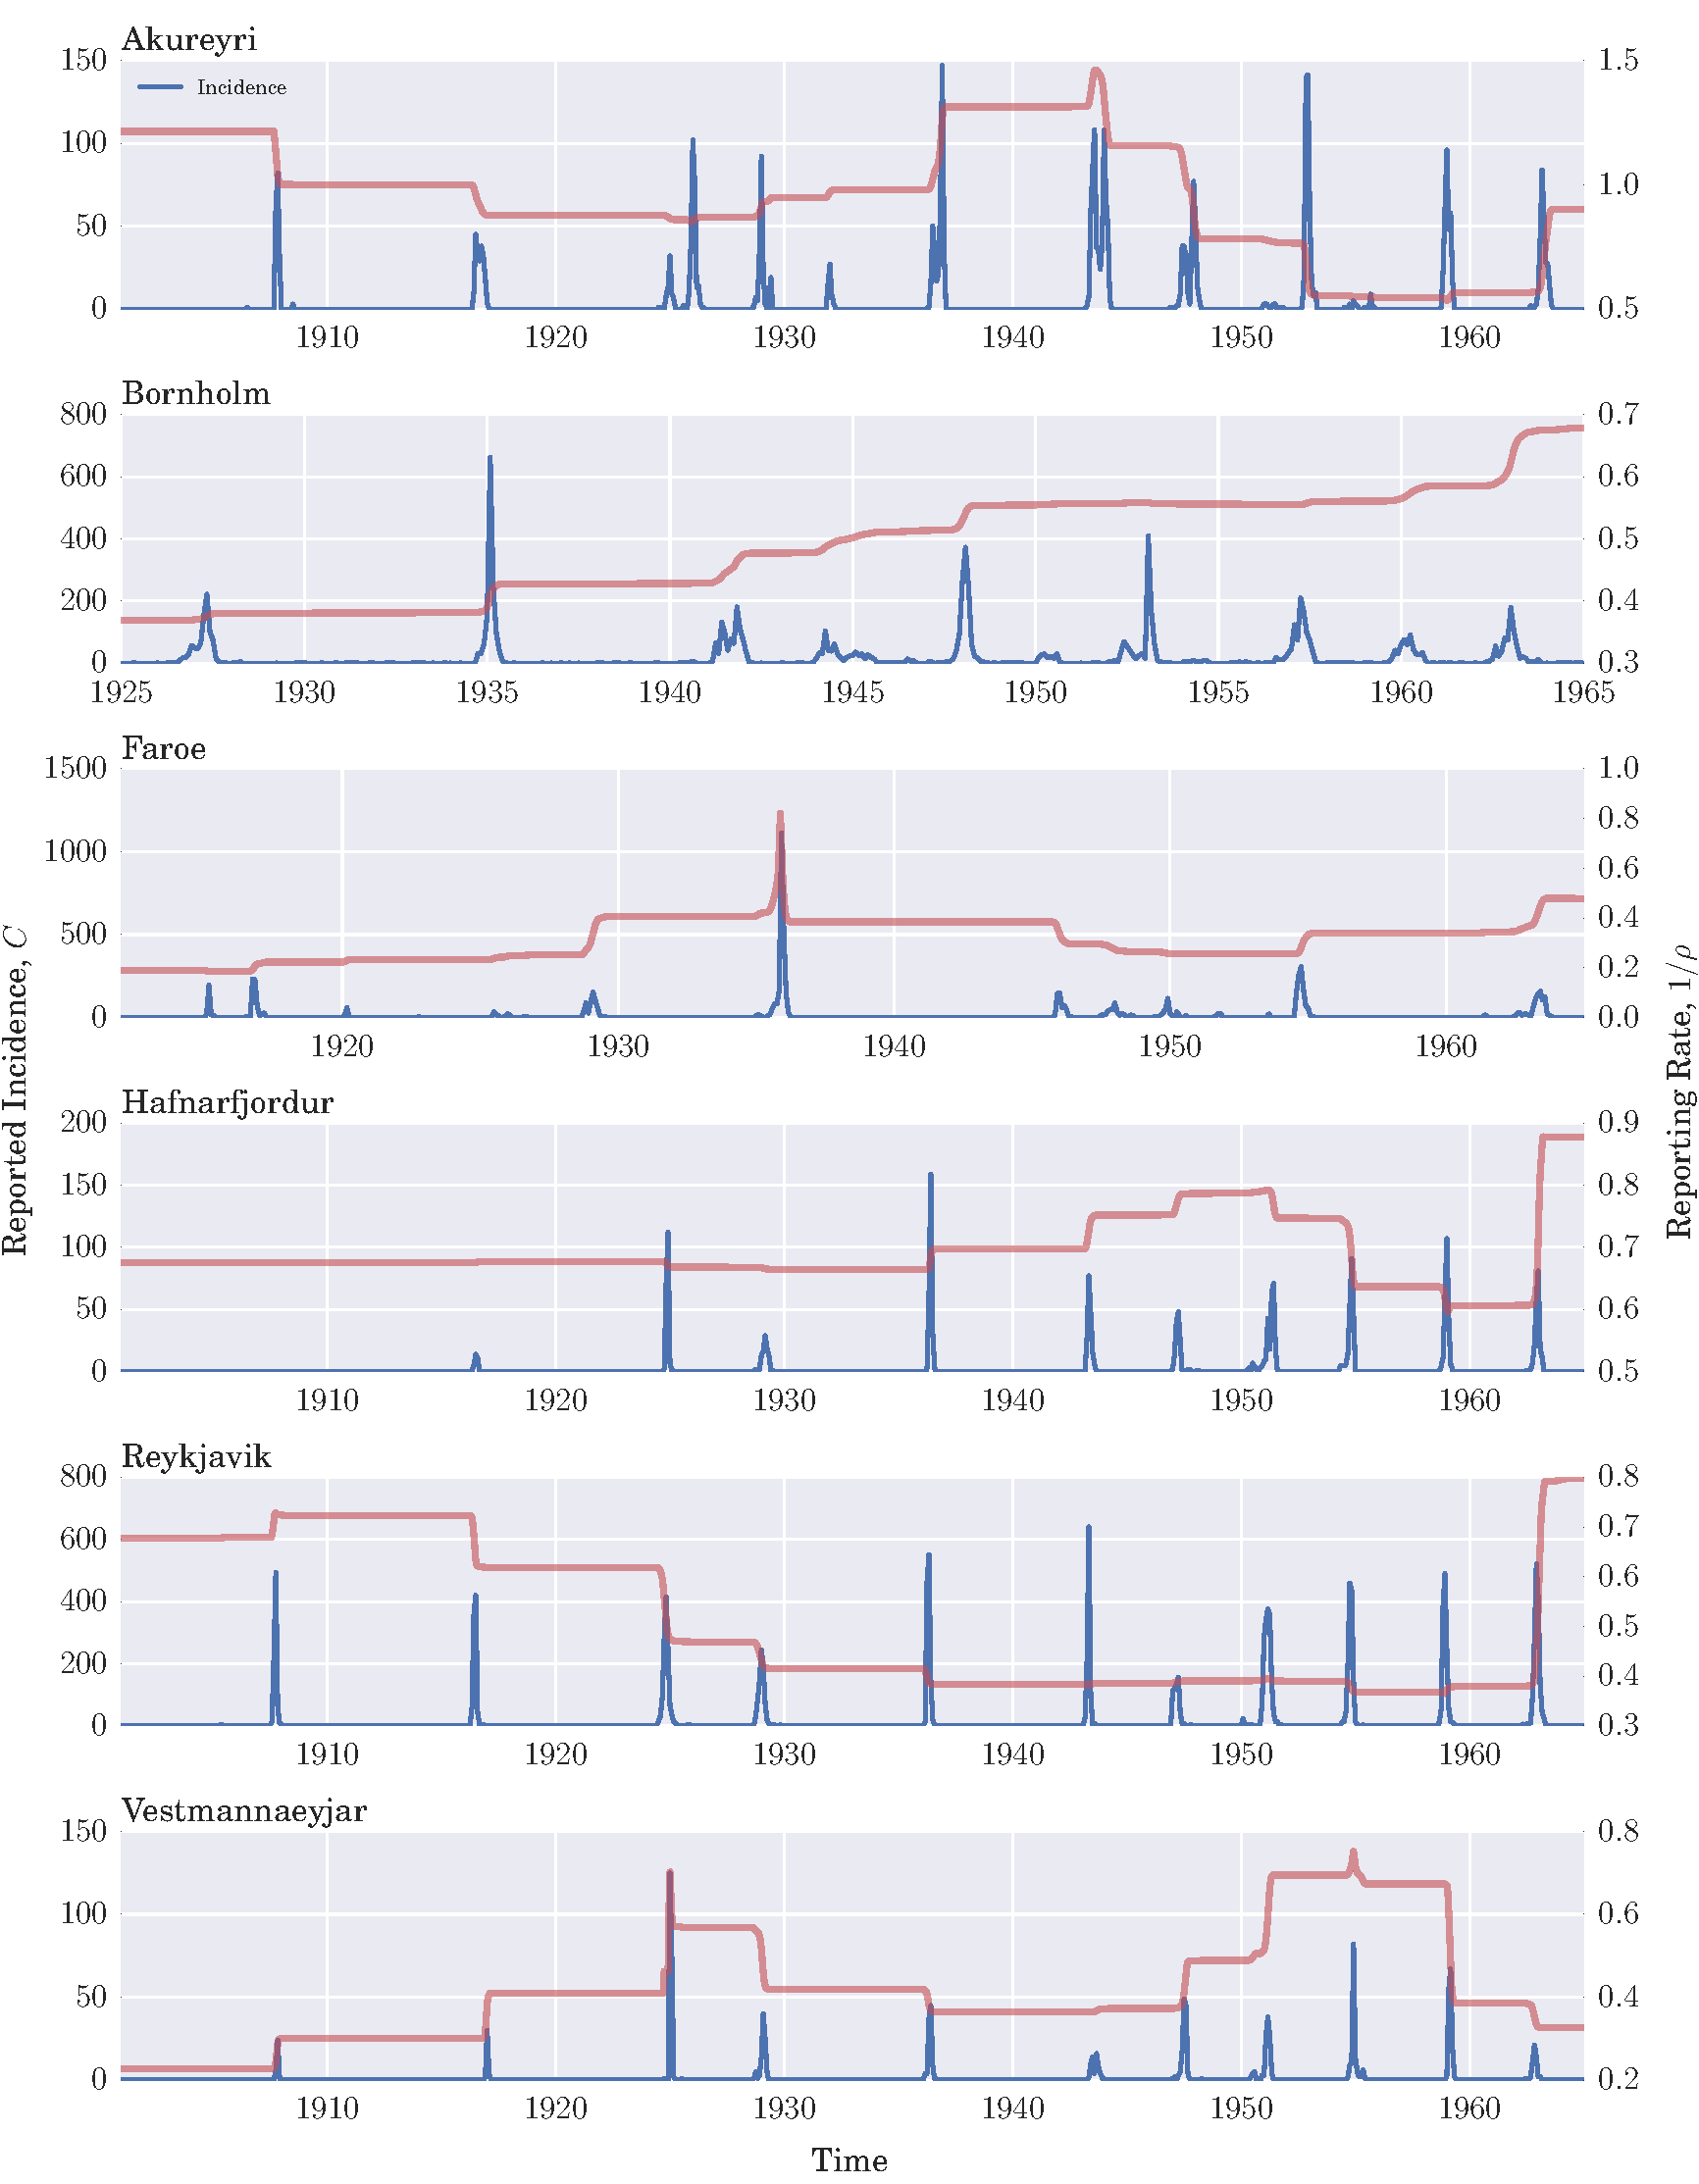
\includegraphics[width=0.9\textwidth]{figures/0_incidence.pdf}
\end{figure}



\begin{figure}[H]
\label{fig_seasonality}
\caption{\textbf{Seasonality.} Numbers reported are $r$ in main TSIR equation ( method section to be written ). Overall notes : magnitude fairly small; effectively flat when considering CIs.}
\centering
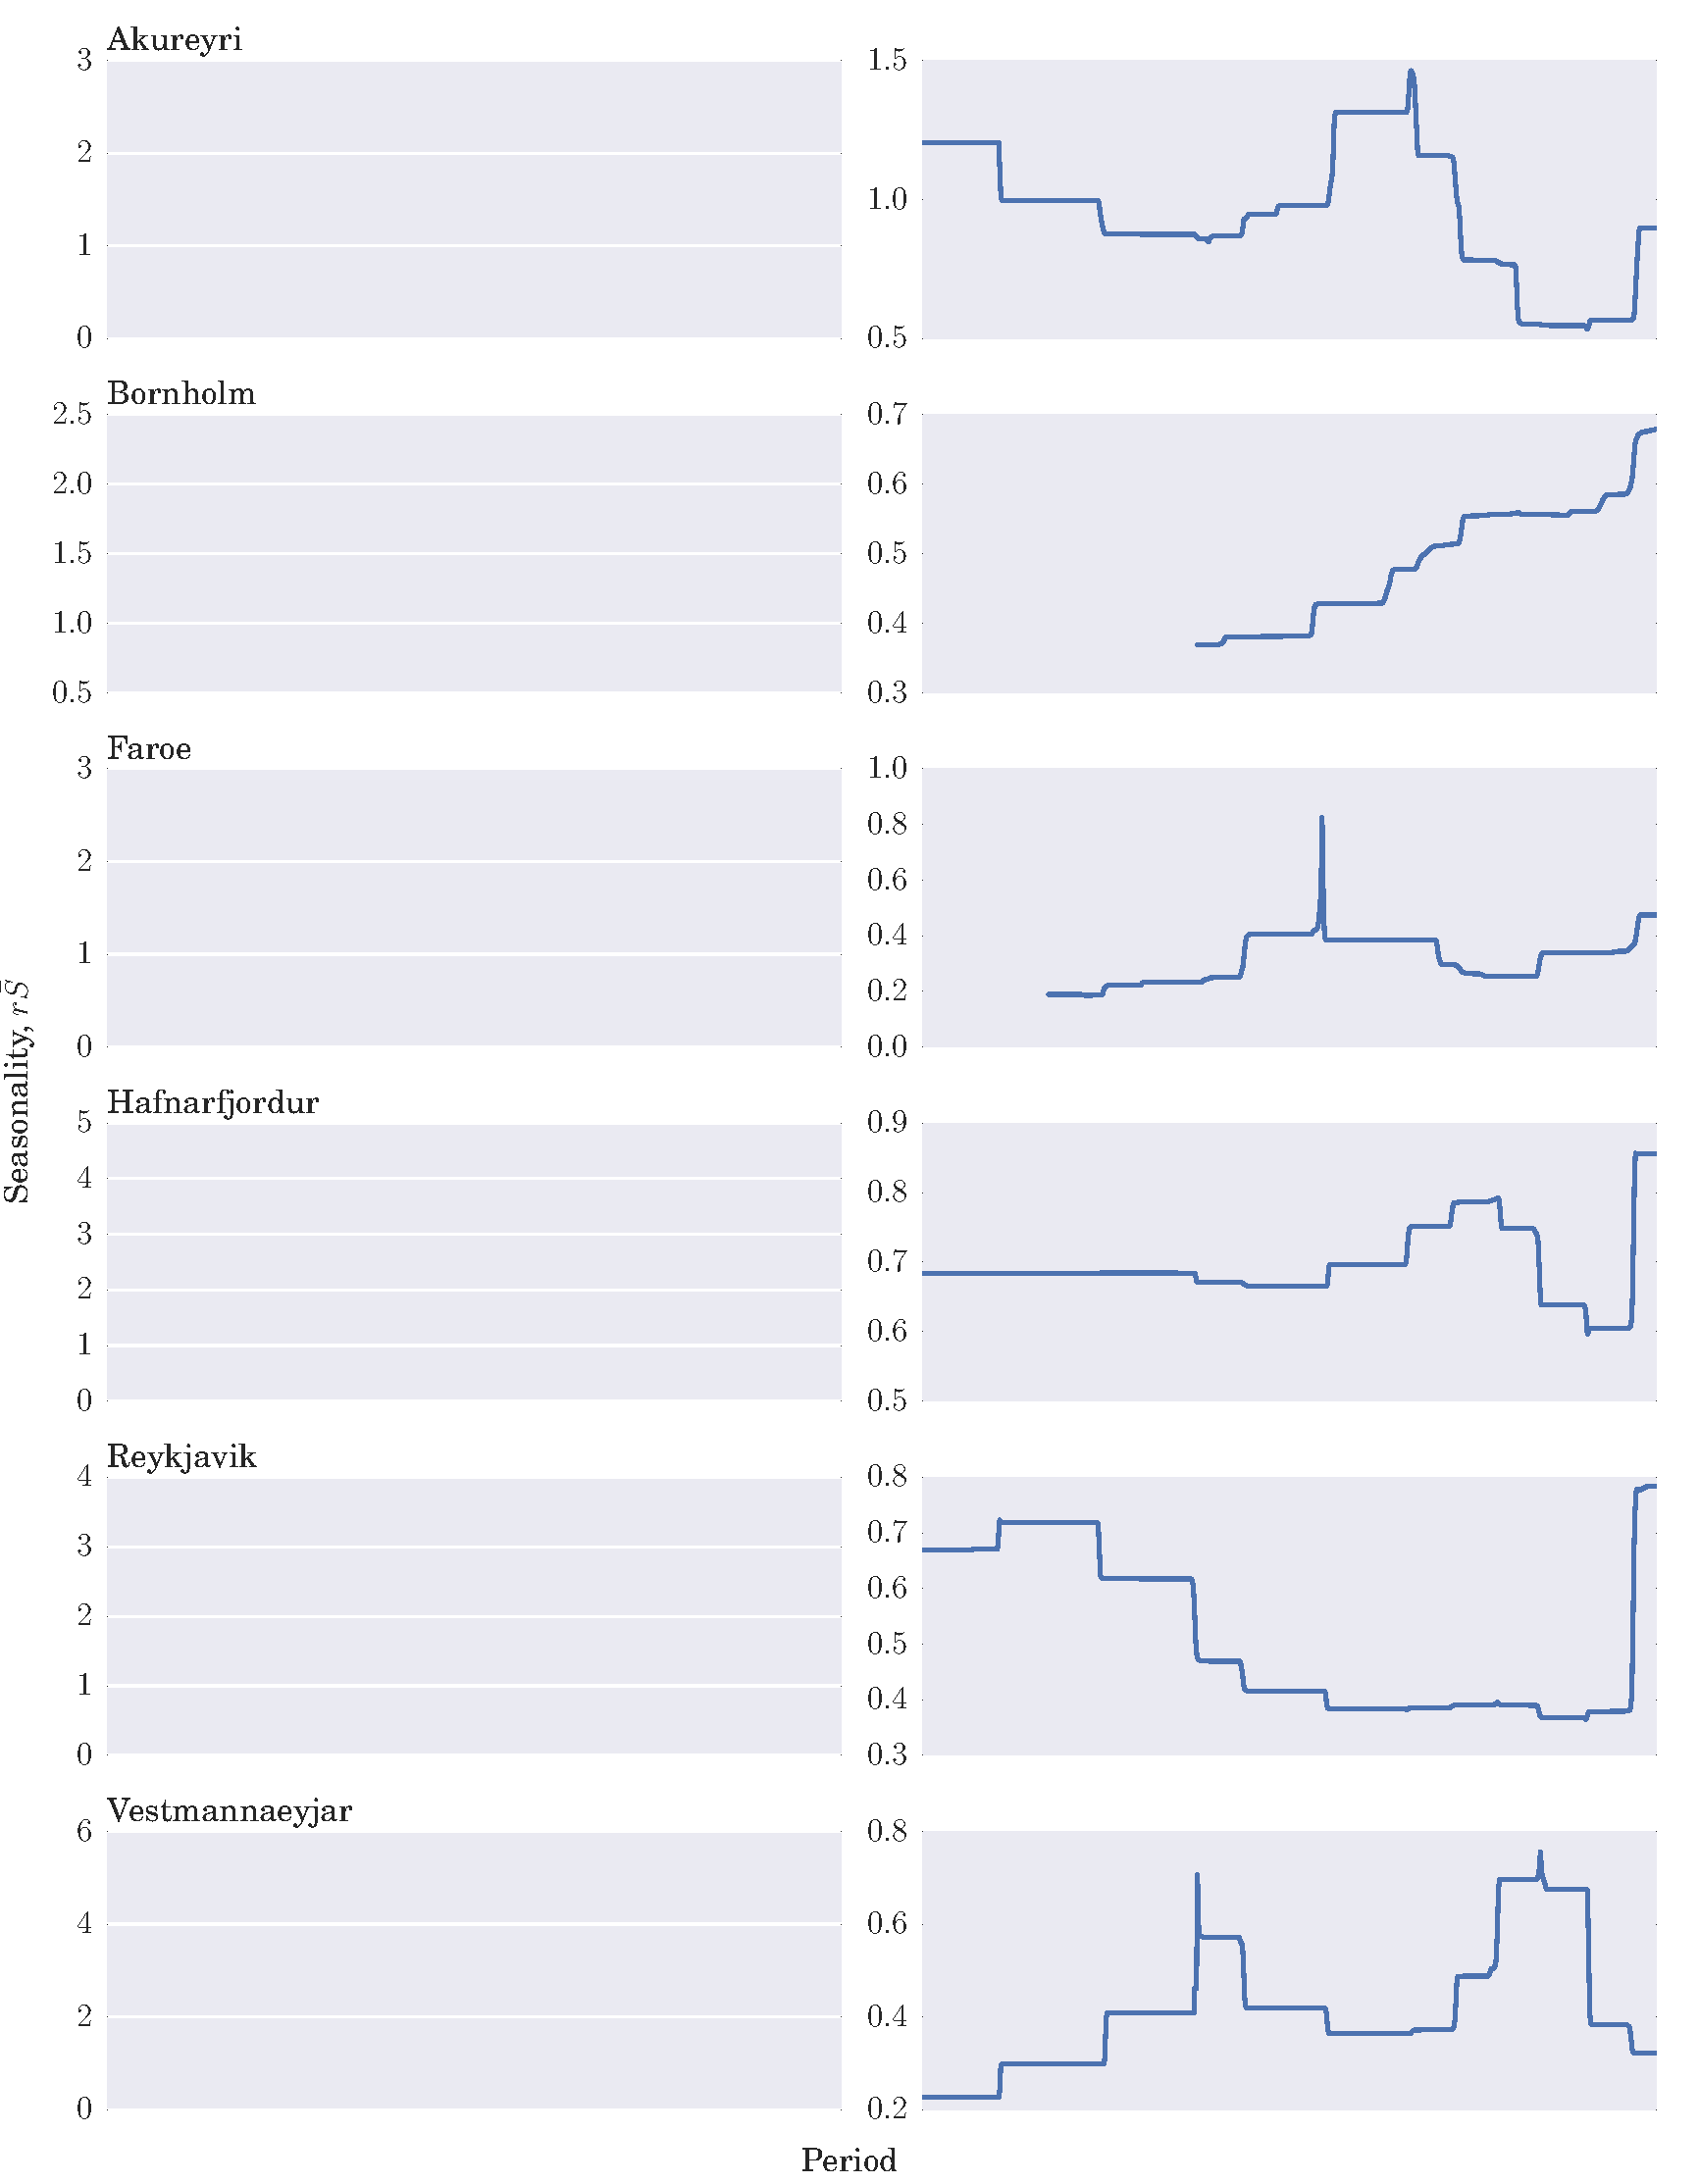
\includegraphics[width=0.9\textwidth]{figures/1_seasonality.pdf}
\end{figure}





\begin{figure}[H]
\label{fig_predictions}
\caption{\textbf{Predictions.} Simulations are conditioned on first time step of an epidemic, and are allowed to run until next epidemic starts. Some reasonable predictions ? Fits better with spikier data (!) when a good, clean epidemic occurs.}
\centering
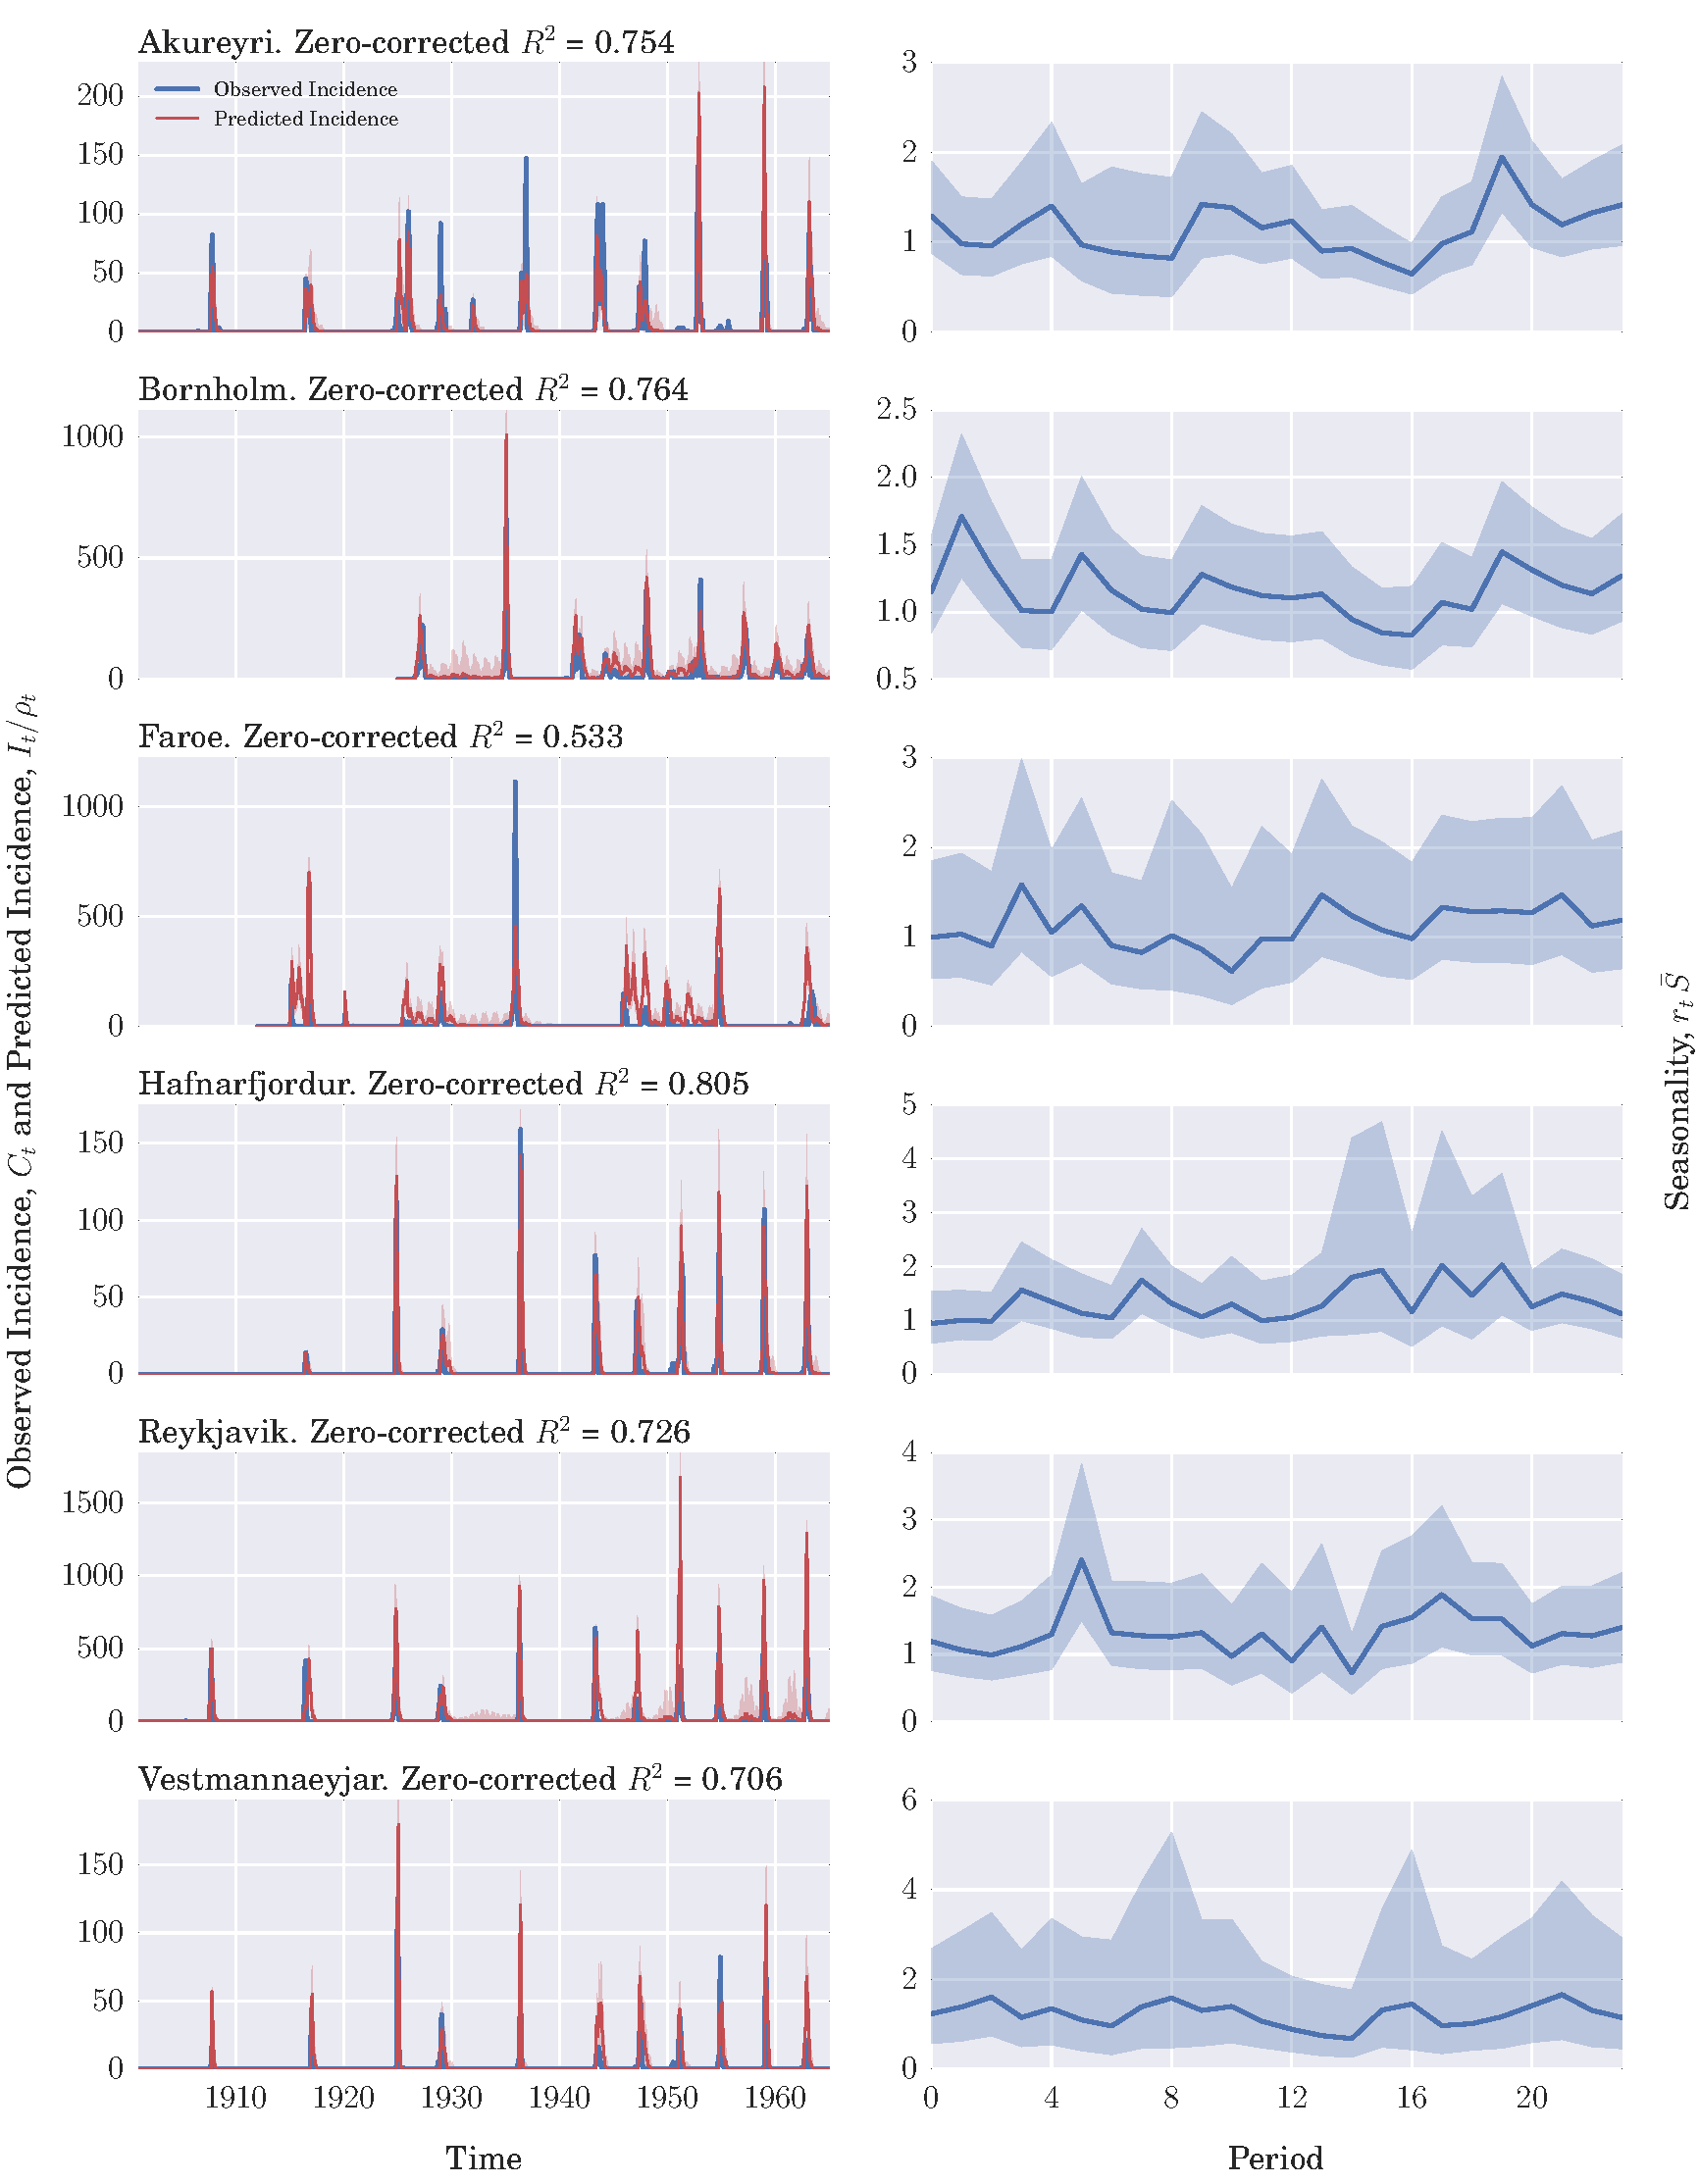
\includegraphics[width=0.9\textwidth]{figures/2_predictions.pdf}
\end{figure}






\begin{figure}[H]
\label{fig_sizes}
\caption{\textbf{Predictability of Epidemic Sizes.} With 10000 simulations. Note Bornholm ( single island, clean data effect ) vs Faroe ( many small islands, aggregate incidence data ) vs Icelandic areas ( disconnected demographics vs incidence borders ). In good locations, we can certainly give a good prediction of epi size. Tend to do better for large epidemics. Gradients all ABOUT one, some slightly over ( right shoulder effect ? ). Large variability in error bars - some epidemics are easier to predict than others ( why ? )}
\centering
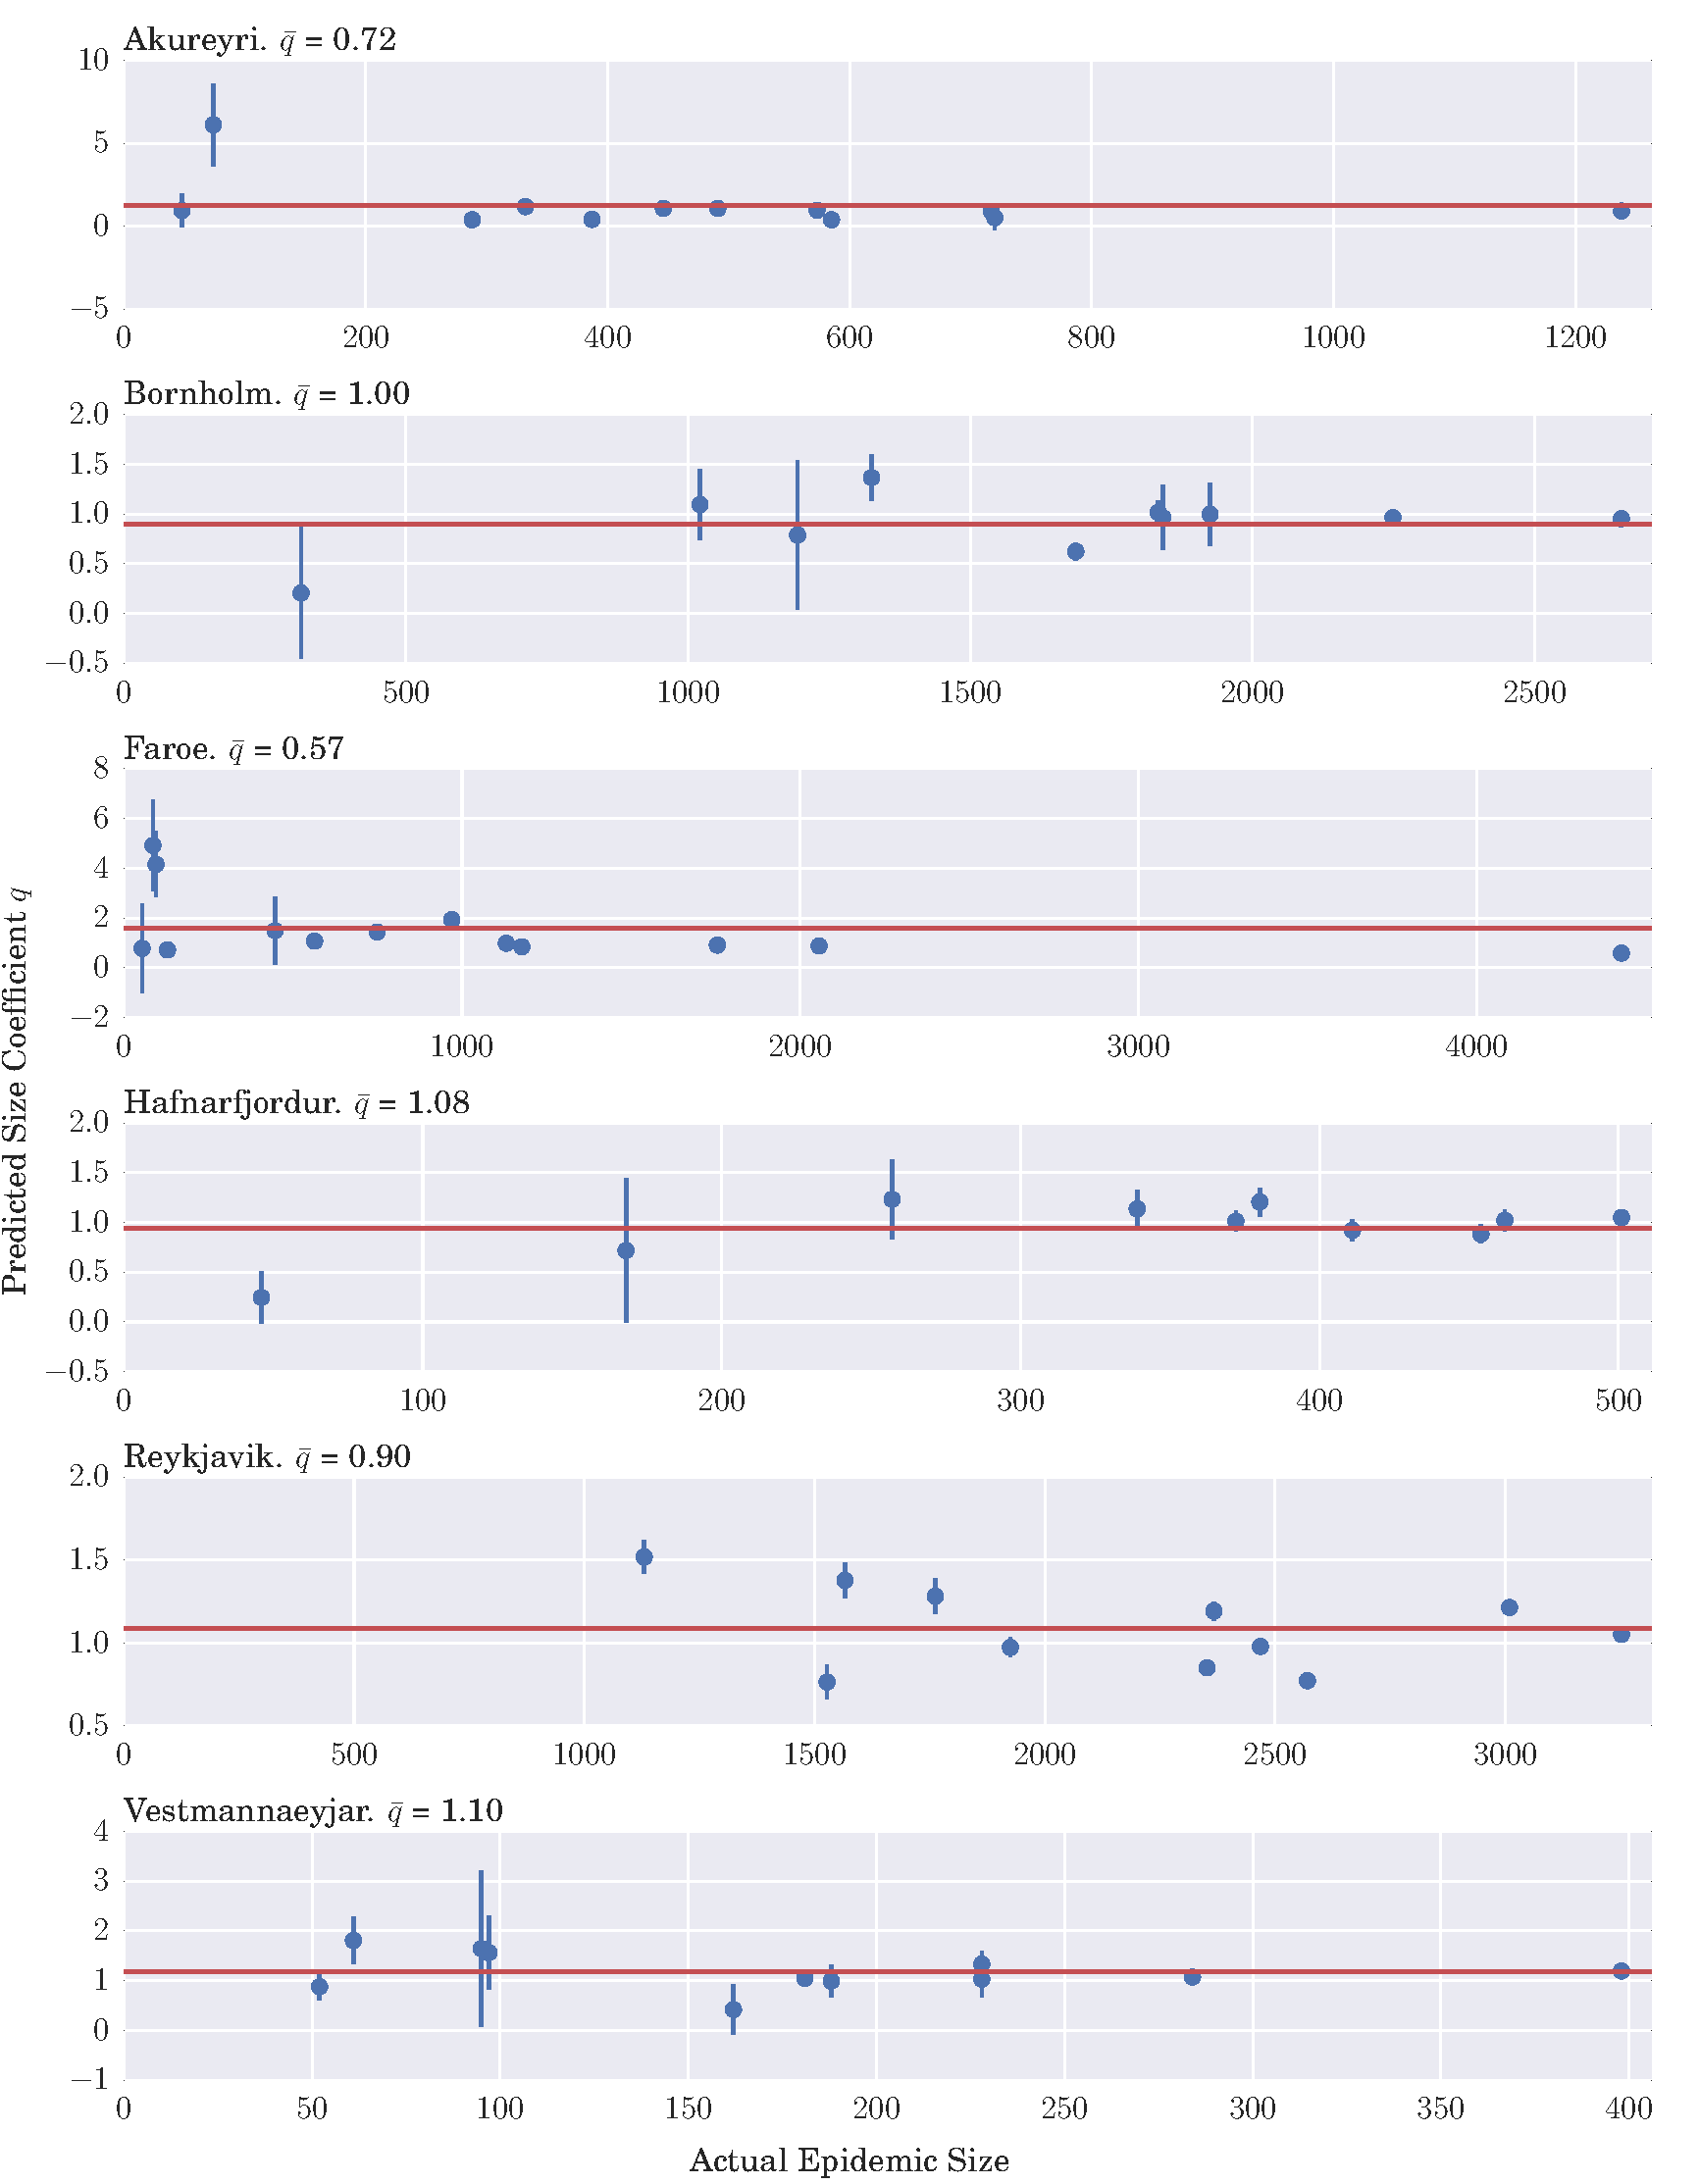
\includegraphics[width=0.9\textwidth]{figures/3_sizes.pdf}
\end{figure}















\section*{Discussion}

Interpolated our monthly data for 24 periods - discuss effects of this. Trajectory matching vs simple interpolation.

Reconstructed susceptibles in six small populations ( discuss Sbar / N ).

Inferred reporting rate - may be indicator of bad dataset if above one ?

Low to no seasonal effects found - do we want a histogram of epidemic periods throughout the year ? No relatable seasonal effects within Iceland. Do we prefer 12-period of 24-period seasonality ? Could $r$ be representative of some simply random effect that is not really a seasonal factor ? Can we do as well in predicting using flat $r$ ?

SOME predictability found - given the simple model, we do OK at reconstructing epidemics. Reasonable correlation between the epidemic sizes. Duration much less predictable - possible due to how we define an epidemic and cut them off as they run into the next one.

In all cases, our epidemics are longer in time - we don't go extinct as much as we should. Can we suggest an improvement in the model to ameliorate this ?

Intercept on size plot - we should be seeing zero intercept, gradient one. We're seeing greater gradient, so we're overestimating size; positive intercept may indicate improvement needed in the model










% You may title this section "Methods" or "Models". 
% "Models" is not a valid title for PLoS ONE authors. However, PLoS ONE
% authors may use "Analysis" 
\section*{Materials and Methods}











% Do NOT remove this, even if you are not including acknowledgments
\section*{Acknowledgments}









%\section*{References}
% The bibtex filename
\bibliography{qbib}

\section*{Figure Legends}
%\begin{figure}[!ht]
%\begin{center}
%%\includegraphics[width=4in]{figure_name.2.eps}
%\end{center}
%\caption{
%{\bf Bold the first sentence.}  Rest of figure 2  caption.  Caption 
%should be left justified, as specified by the options to the caption 
%package.
%}
%\label{Figure_label}
%\end{figure}


\section*{Tables}
%\begin{table}[!ht]
%\caption{
%\bf{Table title}}
%\begin{tabular}{|c|c|c|}
%table information
%\end{tabular}
%\begin{flushleft}Table caption
%\end{flushleft}
%\label{tab:label}
% \end{table}

\end{document}

